\section{Motivating Scenarios}
\label{s:deploy}
%\radhika{need a better title?}

\begin{figure*}
    \centering
    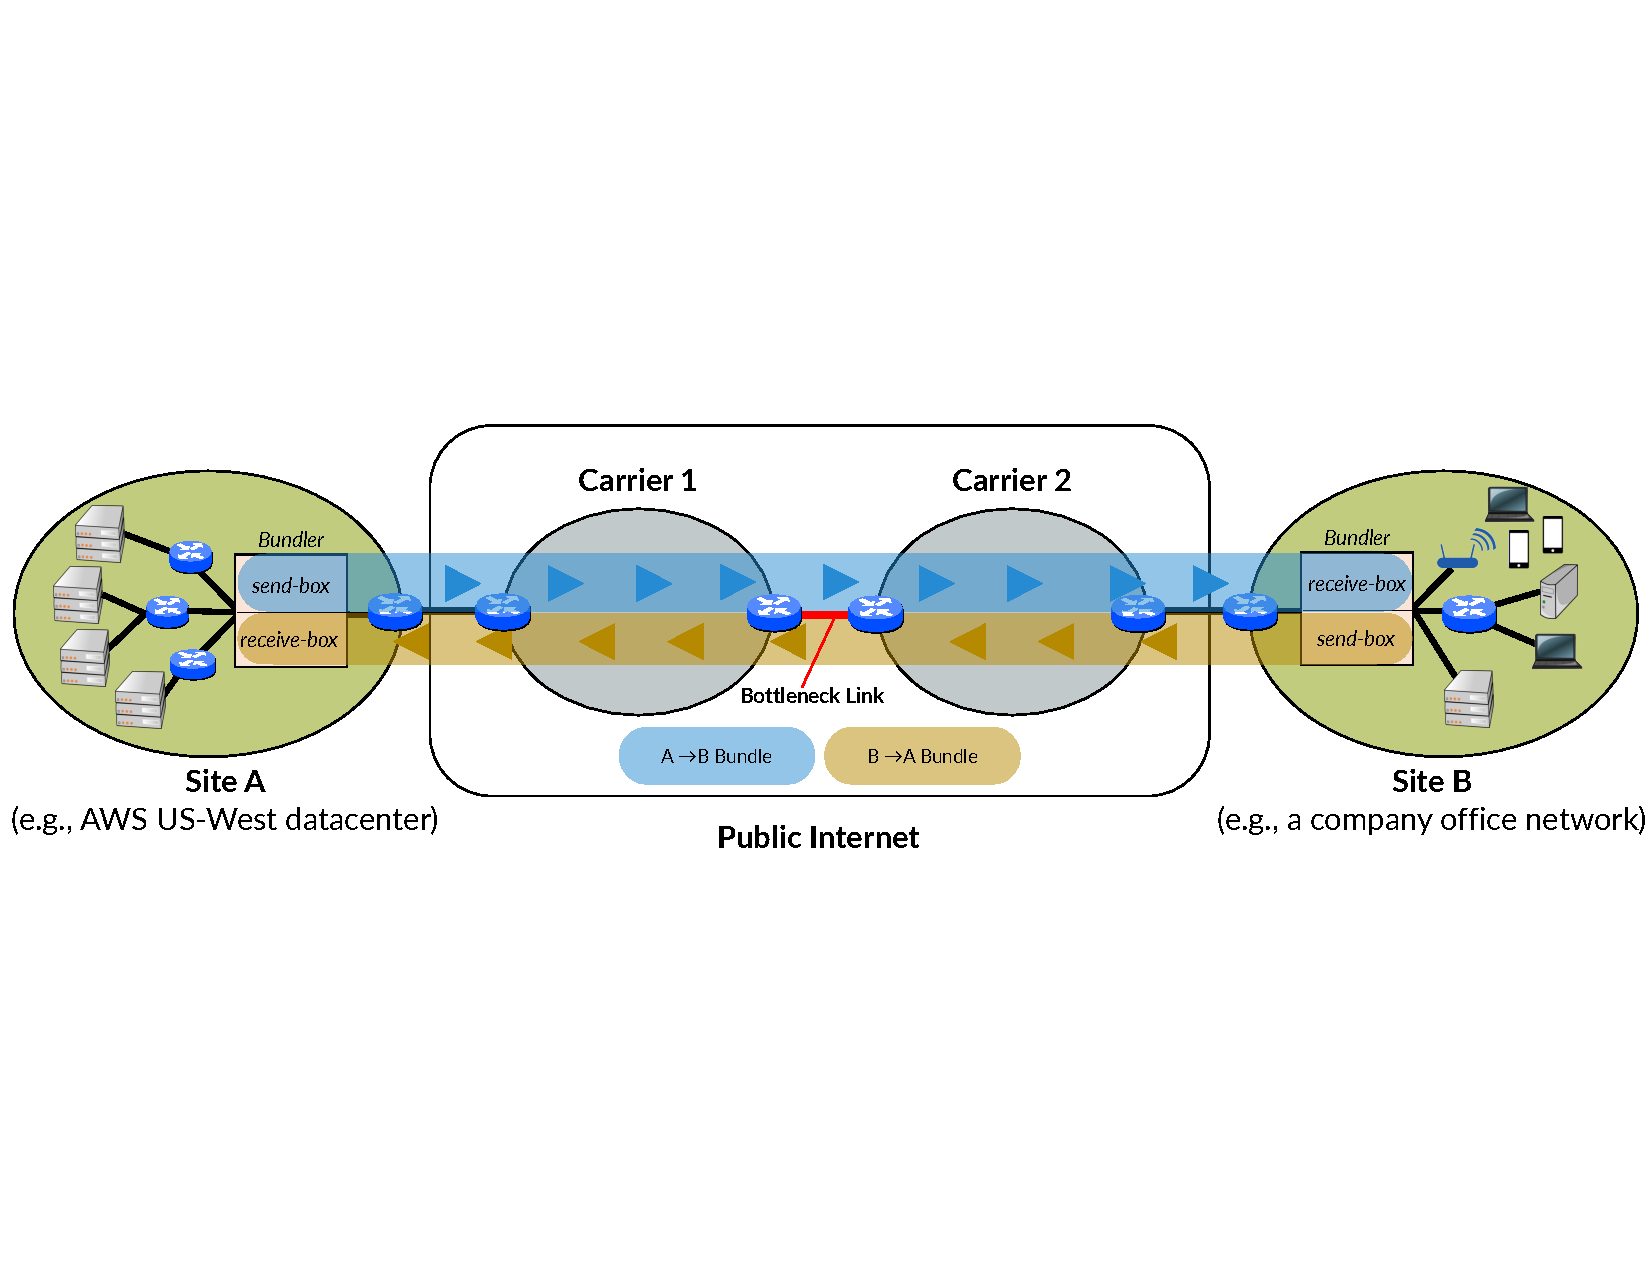
\includegraphics[width=\textwidth]{img/deployment-arch.pdf}
    \caption{An example deployment scenario for \name. 
    The \inbox sits at the sending domain's egress and \outbox sits at the receiving domain's ingress. Bottleneck exists between the \inbox and the \outbox. All traffic between the two boxes gets bundled together. 
    %The solid lines depict links used by the traffic in the bundle, while the dotted lines represent other possible links. 
    }\label{fig:deploy:arch}
\end{figure*}


Figure~\ref{fig:deploy:arch} depicts a representative deployment scenario for \name. The sending domain deploys \name's \inbox at its egress to the public network, while the receiving domain deploys the \outbox at its ingress. All traffic between the \pair is aggregated into the same bundle. The queueing inflicted by the bundled traffic at the bottleneck links in the network is moved to the \inbox, as described in \S\ref{s:design}. The \inbox can then enforce desired scheduling and queue management policies across the traffic in the bundle. 

For the rest of this section, we use a running example of the sending domain belonging to a large content provider (say, \egsender) and the receiving domain being an enterprise network. Similar arguments would hold for the other deployment scenarios (exemplified in \S\ref{s:intro}) as well. 

\vspace{0.05in}

\noindent \name's performance benefits depend on the following: 

\Para{Amount of Aggregation} 
Since \name schedules packets across flows within a given bundle, its performance benefits would increase with the number of such aggregated flows, due to increase in scheduling opportunities. So the natural question to ask is, would we have sufficient amount of aggregation in practice to make a \name deployment beneficial? 

Recent observations~\cite{fivecomps} \radhika{find other cites} do indicate a positive response to this question. This is driven by the fact that majority of traffic across the Internet today is owned by a few large content providers who provide a wide array of services. In our example scenario, a bundle could thus comprise of significant amount traffic generated by \egsender's various services (such as email, messaging, video conferencing, video streaming, cloud storage etc.) for different clients within the enterprise.



% \begin{itemize}
%     \item Cite venkat's hotnets and Labovitz paper (any other citations?)
% \end{itemize}

\Para{Shared bottleneck in the middle of the network} \name can move queues (and therefore gain scheduling power) only from the bottleneck links in the middle of the network, i.e. between a \pair. So the next question that arises is, would a bottleneck occur in the middle of the network, in practice? We observe that this can indeed be the case under the following scenarios:

\paragraphi{Rate Limiting} Bandwidth throttling by ISPs has become a common practice~\cite{isp-throttle-1, isp-throttle-2, isp-throttle-3}. Consequently, bottlenecks may arise at the peering links of different carrier networks (shown in red in Figure~\ref{fig:deploy:arch}), and particularly at the links connecting the last-hop ISPs to the receiving domains. Such bottlenecks can result in a queue build up due the flows in a single bundle (which we call self-inflicted queueing), even in the absence of any other cross-traffic. 

\paragraphi{When carriers do rate limiting}
Find citations
\begin{itemize}
    \item can result in self-inflicted bottlenecks (any citations to show how common this is?).
    \item best case for bundler.
\end{itemize}

\paragraphi{Congestion from other traffic}
\begin{itemize}
    \item short-lived (up to a few MB) cross traffic: we still get benefits.
    \item other bundled traffic: we still get benefits.
    \item long-lived persistent connections: fall back to status quo.
\end{itemize}
\radhika{Also say something about placement of \inbox \outbox pairs.}

%\Para{Bottleneck is shared by the bundled traffic}